\documentclass[a4paper,12pt]{article} 
\usepackage{geometry}
\usepackage{wrapfig}
\geometry{
	a4paper,
	total={170mm,257mm},
	left=10mm,
	right=10mm,
	top=20mm,
}
\usepackage{titlesec}
\titlelabel{\thetitle.\quad} %точка в section

%%% Работа с русским языком
\usepackage{cmap}                           % поиск в PDF
\usepackage{mathtext} 			 	       % русские буквы в формулах
\usepackage[T2A]{fontenc}               % кодировка
\usepackage[utf8]{inputenc}              % кодировка исходного текста
\usepackage[english,russian]{babel}  % локализация и переносы

\usepackage{indentfirst}
\usepackage[pdftex]{graphicx}
\usepackage{multirow}
\usepackage{biblatex}
\usepackage{siunitx}
\usepackage{subcaption,floatrow,graphicx,calc}
\usepackage{fancyhdr}

%Математика
\usepackage{amsmath,amsfonts,amssymb,amsthm,mathtools} % AMS
\usepackage{icomma} % "Умная" запятая

%% Шрифты
\usepackage{euscript}	 % Шрифт Евклид
\usepackage{mathrsfs} % Красивый матшрифт

\usepackage{gensymb}
\usepackage{graphicx}
\usepackage{setspace}
\usepackage{tabularx}
\usepackage{longtable}
\usepackage{euscript}
\usepackage{float}
\usepackage{cutwin}
\usepackage{adjustbox}
\usepackage{dashbox}
\usepackage[normalem]{ulem}	
\usepackage[babel=true]{microtype}
\RequirePackage[T1]{fontenc}
\usepackage{amsmath,amsfonts,amssymb,amsthm,mathrsfs,mathtools} 
\usepackage{xcolor}         
\usepackage{enumitem}     
\usepackage{xpatch}       
\usepackage{cancel}                  
\usepackage{upgreek}                 
\usepackage{lipsum}                  
\usepackage[version=4]{mhchem}       
\usepackage{multirow}                
\usepackage{stackengine}             
\usepackage{tikz}         
\usepackage{hyperref}
\hypersetup{colorlinks=true,urlcolor=blue}       
\usetikzlibrary{positioning}         
\usepackage{titletoc}                 
\usepackage{chngcntr}              
\usepackage{fancyhdr}                
\usepackage{makecell}                
\usepackage{indentfirst}             
\usepackage{tocloft}                 
\usepackage{soul}                   
\usepackage[stable]{footmisc}       
\usepackage{subfig}  
\usepackage{comment}                  


\mathtoolsset{showonlyrefs=true}


\theoremstyle{definition}
\newtheorem*{definition}{Определение}
\newtheorem{statement}{Предложение}[section]
\newtheorem{lemma}{Лемма}[section]
\newtheorem{theorem}{Теорема}[section]
\newtheorem*{theoremn}{Теорема}
\newtheorem*{corollary}{Следствие}
\newtheorem*{example}{Пример}
\newtheorem*{note}{Замечание}
\newtheorem*{problem}{Задача}


\counterwithout{footnote}{section}\DeclareRobustCommand{\divby}{%
	\mathrel{\text{\vbox{\baselineskip.65ex\lineskiplimit0pt\hbox{.}\hbox{.}\hbox{.}}}}%
}

\newcommand{\dotpr}[2]{\bra{#1}\ket{#2}}
\let\AA\relax
\let\emptyset\varnothing
\DeclareMathOperator*{\esssup}{ess sup}
\DeclareMathOperator*{\ord}{ord}
\DeclareMathOperator*{\supp}{supp}
\DeclareMathOperator*{\pr}{pr}
\DeclareMathOperator*{\Ker}{Ker}
\DeclareMathOperator*{\Vol}{Vol}
\DeclareMathOperator*{\rg}{rk}
\DeclareMathOperator*{\Ima}{Im}
\DeclareMathOperator*{\Alt}{Alt}
\DeclareMathOperator*{\Sym}{Sym}
\newcommand{\eqdef}{\stackrel{\text{\tiny{def}}}{=}}
\newcommand{\pp}{\partial}
\newcommand{\AA}{\mathcal{A}}
\newcommand{\BB}{\mathcal{B}}
\newcommand{\MM}{\mathbb{M}}
\newcommand{\NN}{\mathbb{N}}
\newcommand{\ZZ}{\mathbb{Z}}
\newcommand{\QQ}{\mathbb{Q}}
\newcommand{\RR}{\mathbb{R}}
\newcommand{\CC}{\mathbb{C}}
\newcommand{\FFF}{\mathbb{F}}
\newcommand{\DD}{\mathcal{D}}
\newcommand{\FF}{\mathcal{F}}
\newcommand{\sS}{\mathcal{S}}
\newcommand*\circled[1]{\tikz[baseline=(char.base)]{
		\node[shape=circle,draw,inner sep=2pt] (char) {#1};}}
\bibliography{bib}
\newcommand{\const}{\mathrm{const}}
\newcommand{\rref}[1]{(\ref{#1})}
\newcommand{\isotope}[2]{$ ^{#2}\mathrm{#1} $}
\newcommand{\picref}[1]{рис. \ref{#1}}
\newcommand{\mbf}{\mathbf}
\newcommand{\gmm}{$\gamma $}
\newcommand{\btt}{$\beta $}
\newcommand{\dlt}{$\delta $}
	
\title{Лабораторная работа 5.4.2 \\
	\textbf{Исследование энергетического спектра \btt-частиц и определение их максимальной энергии при помощи	магнитного спектрометра}}
\author{Шерхалов Денис Б02-204и \\
		Фаттахов Марат Б02-204кт}
	\date{\today}

\begin{document}
		
	{\Large \maketitle}

	\textbf{В работе}: проводится исследование энергетического	спектра \btt-частиц при распаде ядер \isotope{Cs}{137} и определяется их максимальная энергия. Калибровка спектрометра осуществляется по энергии электронов внутренней конверсии \isotope{Cs}{137}.
	
	\section{Введение}
	
	\begin{wrapfigure}{}{0.49\textwidth}
		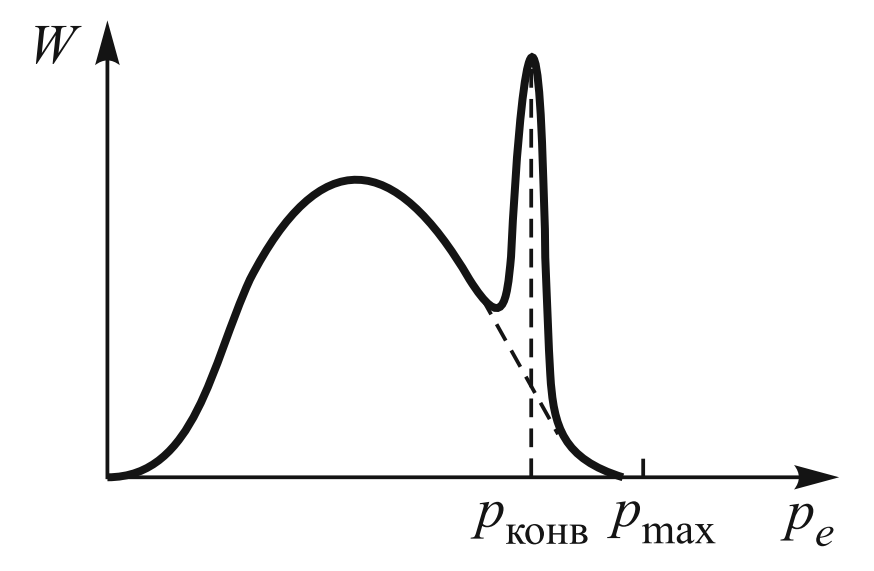
\includegraphics[width=1.0\linewidth]{Screenshot_1}
		\caption{Форма спектра \btt-частиц при разрешённых переходах}
		\label{fig:screenshot1}
	\end{wrapfigure}
	
	Бета-распадом называется самопроизвольное превращение ядер,	при котором их массовое число нс изменяется, а заряд увеличивается или уменьшается на единицу.В данной работе мы будем иметь дело с электронным \btt-распадом:
	\begin{equation*}
		^A_Z X \leftarrow ^A_{Z+1} X+e^-+\widetilde{\nu},
	\end{equation*}
	при котором кроме электрона испускается антинейтрино. 
	
	Выясним вид энергетического спектра \btt-частиц.
	Во-первых, учтём ЗСЭ:
	\begin{equation}\label{eq:ЗСЭ}
		E_e - E - c k = 0,
	\end{equation}
	где $ c k $ -- энергия нейтрино, $ E_e $ -- максимальная энергия электрона, $ E $ -- кинетическая энергия электрона, а связь между его энергией и импульсом даётся соотношением:
	\begin{equation}\label{eq:E}
		E = c \sqrt{p^2+m^2 c^2} - m c^2.
	\end{equation}
	Условие \eqref{eq:ЗСЭ} можно учесть, введя \dlt-функцию вида
	\begin{equation*}\label{key}
		F = \delta(E_e - E - c k),
	\end{equation*}
	которая по определению не равна нулю только если \eqref{eq:ЗСЭ} выполнено.
	Тогда записать вероятность, что электрон после распада имеет импульс $ d^3 p $, а нейтрино --- $ d^3 k $, можно следующим образом:
	\begin{equation}\label{eq:вероятн}
		d w = D \delta(E_e - E - c k) d^3 p d^3 k = D \delta(E_e - E - c k) p^2 d p k^2 d k d \Omega_e d \Omega_{\widetilde{\nu}},
	\end{equation}
	где $ D $ -- коэффициент пропорциональности, который в этом опыте можно считать константой, $ d \Omega_e $ и $ d \Omega_{\widetilde{\nu}} $ -- элементы телесных углов вылета электрона и нейтрино.
	
	Вероятность искомого события имеет связь со спектром, так как
	\begin{equation}\label{eq:связь_спектра_и_вероятн}
		d N = N_0 d w.
	\end{equation}
	Тогда интегрируем \eqref{eq:вероятн} и учитываем \eqref{eq:связь_спектра_и_вероятн}:
	\begin{equation*}\label{eq:dN}
		d N = \dfrac{16 \pi^2 N_0}{c^2} D p^2 \left(E_e - E\right)^2 d p.
	\end{equation*}
	Дифференцируя \eqref{eq:E}, найдём
	\begin{equation*}\label{key}
		d E = \dfrac{c^2 p}{E+m c^2}d p.
	\end{equation*}
	Тогда окончательно
	\begin{equation}\label{eq:spectre}
		\dfrac{d N}{d E} = N_0 B \sqrt{E\left(E+2 m c^2\right)}\left(E_e-E\right)^2\left(E+m c^2\right), 
	\end{equation}
	что в нерелятивистском приближении упрощается до 
	\begin{equation}\label{eq:simpleSpectre}
		\dfrac{d N}{d E} \approx \sqrt{E} \left(E_e - E\right)^2.
	\end{equation}
	
	Дочерние ядра, возникающие в результате \btt-распада, нередко оказываются возбужденными. Возбужденные ядра отдают свою энергию	либо излучая \gmm-квант, либо передавая избыток энергии одному из электронов с внутренних оболочек атома. Излучаемые в таком	процессе электроны имеют строго определенную энергию и называются конверсионными.
	Соответствующий спектр отображён на рис. \ref{fig:screenshot1}.
		
	\subsection*{Оборудование и инструментальные погрешности}
		
	Схема экспериментальной установки отображена на рис. \ref{fig:screenshot2} и \ref{fig:screenshot3}.
	\begin{figure}
		\centering
		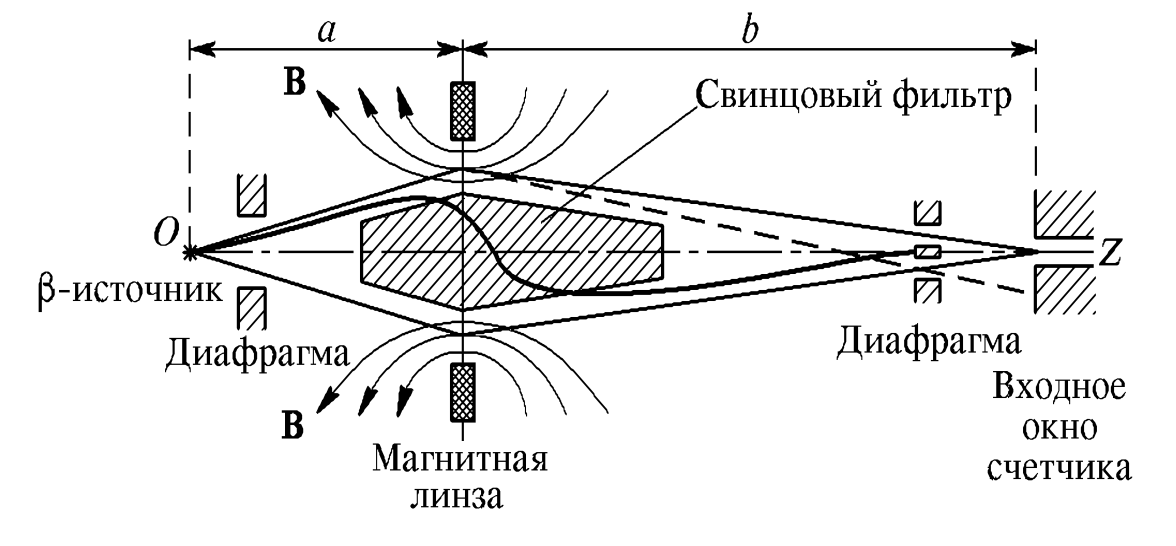
\includegraphics[width=0.7\linewidth]{Screenshot_2}
		\caption{Схема магнитной линзы}
		\label{fig:screenshot2}
	\end{figure}
	\begin{figure}
		\centering
		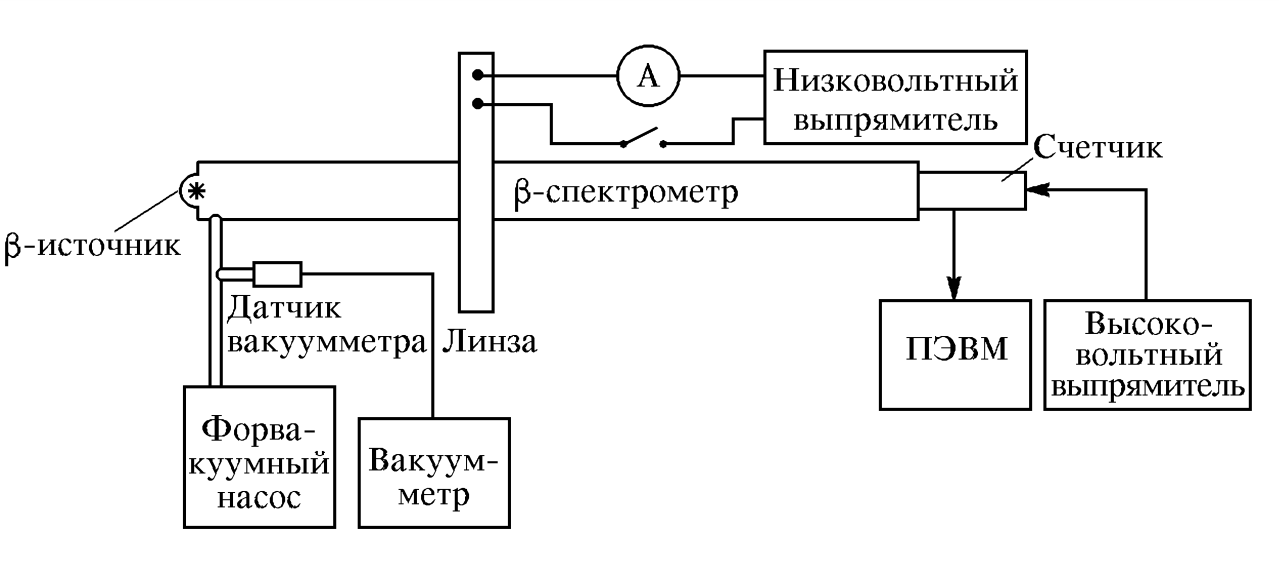
\includegraphics[width=0.7\linewidth]{Screenshot_3}
		\caption{Блок-схема экспериментальной установки}
		\label{fig:screenshot3}
	\end{figure}
	При заданной силе тока на входное окно счетчика фокусируются электроны с определенным импульсом. Электроны, обладающие другими значениями импульса, при этом не сфокусированы и в основном проходят мимо окна. При изменении тока в катушке на счетчик последовательно фокусируются электроны с разными	импульсами, то есть
	\begin{equation*}\label{eq:impulse}
		p_e = k I,
	\end{equation*}
	где $ I $ -- ток катушки.
	Для числа электронов, имеющих импульс $ p_e+\Delta p_e $, можно получить
	\begin{equation*}\label{eq:n_ot_Pe}
		N(p_e) = C W(p_e) p_e,
	\end{equation*}
	где $ C = \const $, $ W(p_e) = d w / d p_e $ находится из формулы \eqref{eq:simpleSpectre}.
	

	В работе используются:
	\begin{itemize}
		\item{\btt-источник}
		\item{Форвакуумный насос}
		\item{Вакуумметр (фигура номинальная)}
		\item{Магнитная линза со свинцовым фильтром и диафрагмой}
		\item{Сцинтилляционный счётчик}
		\item{Источники питания}{0,02}{А}
		\item{Компьютер}
	\end{itemize}
	
	\section{Обработка результатов}
		По результатам измерений построим график cпектра $\beta$-распада атома $^{137}$Cs и откалибруем его.
        Сдвиг графика по оси ординат сделаем на величину радиационного фона $N_\text{ф}$.
		\begin{figure}[h!]
			\begin{floatrow}
				\ffigbox[\FBwidth]{\caption{Спектр $\beta$-распада атома $^{137}$Cs.}\label{fig:spectre1}}%
				{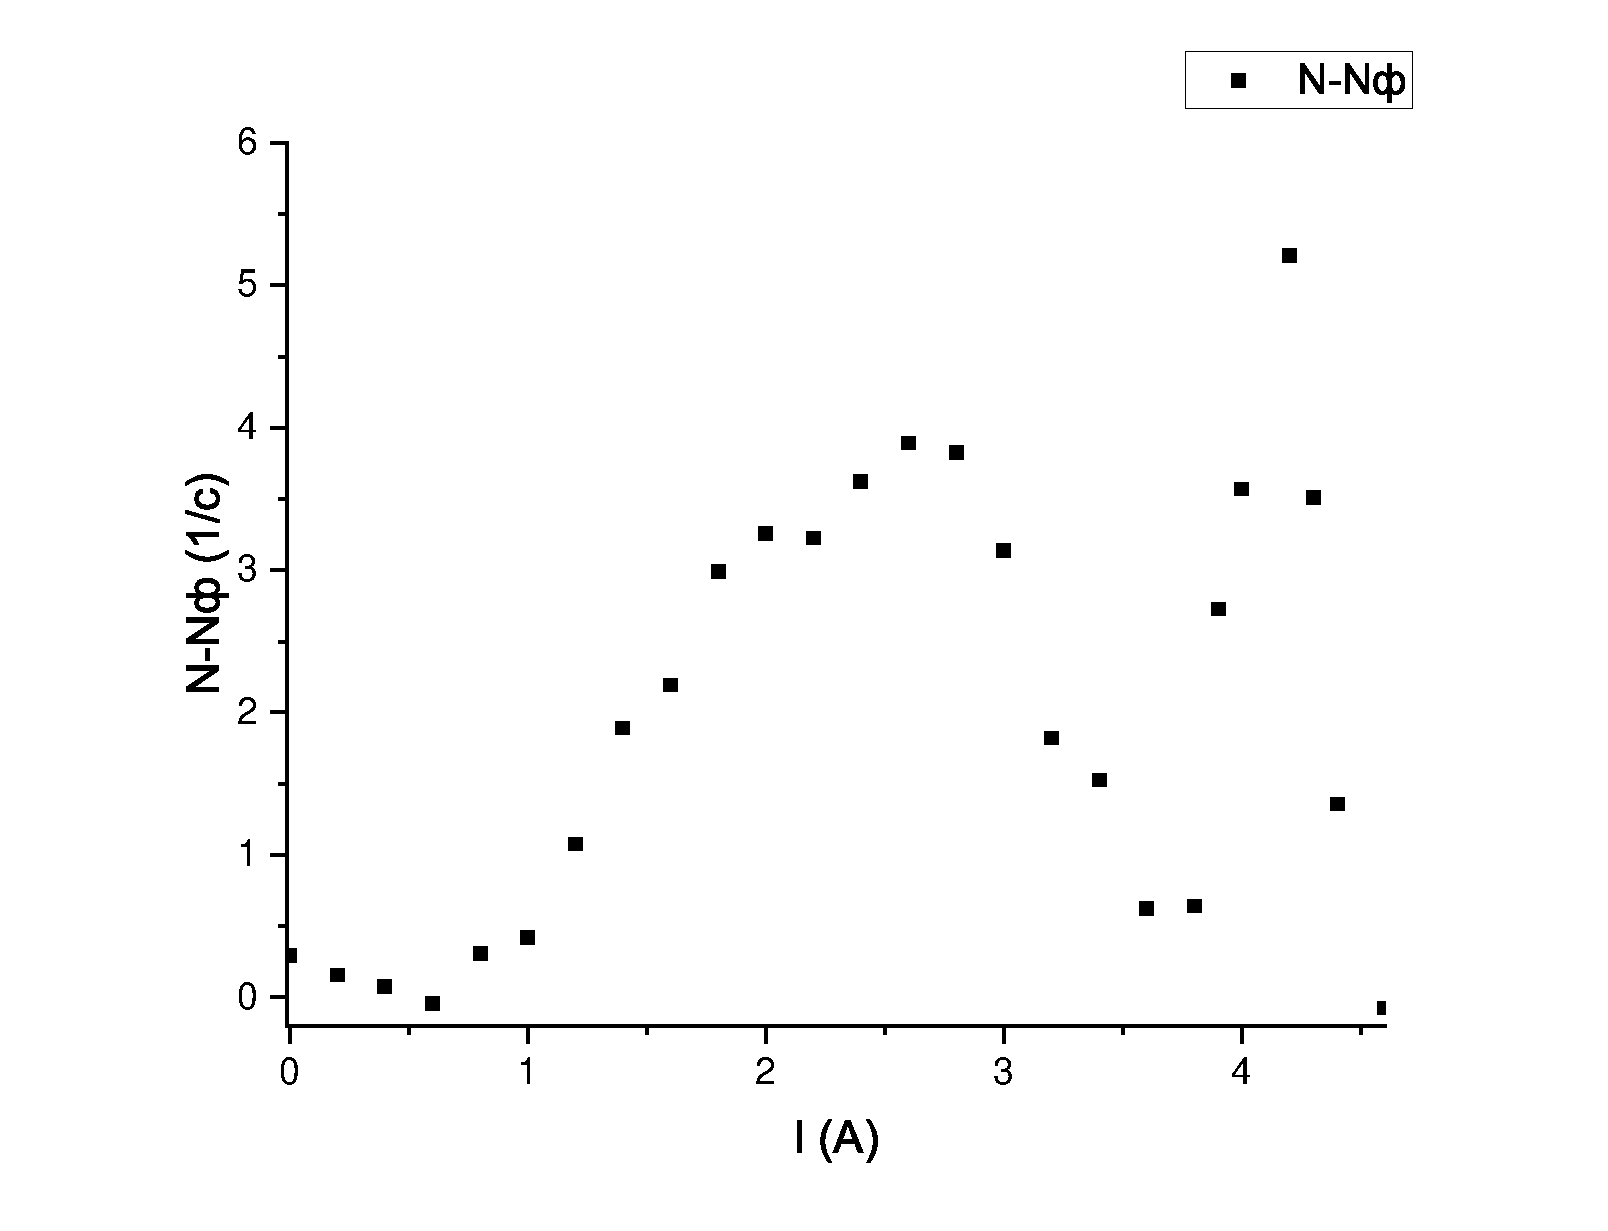
\includegraphics[width=8cm,height=7cm]{Graph1.pdf}}
				\ffigbox[\FBwidth]{\caption{Откалиброванный график.}\label{fig:spectre2}}%
				{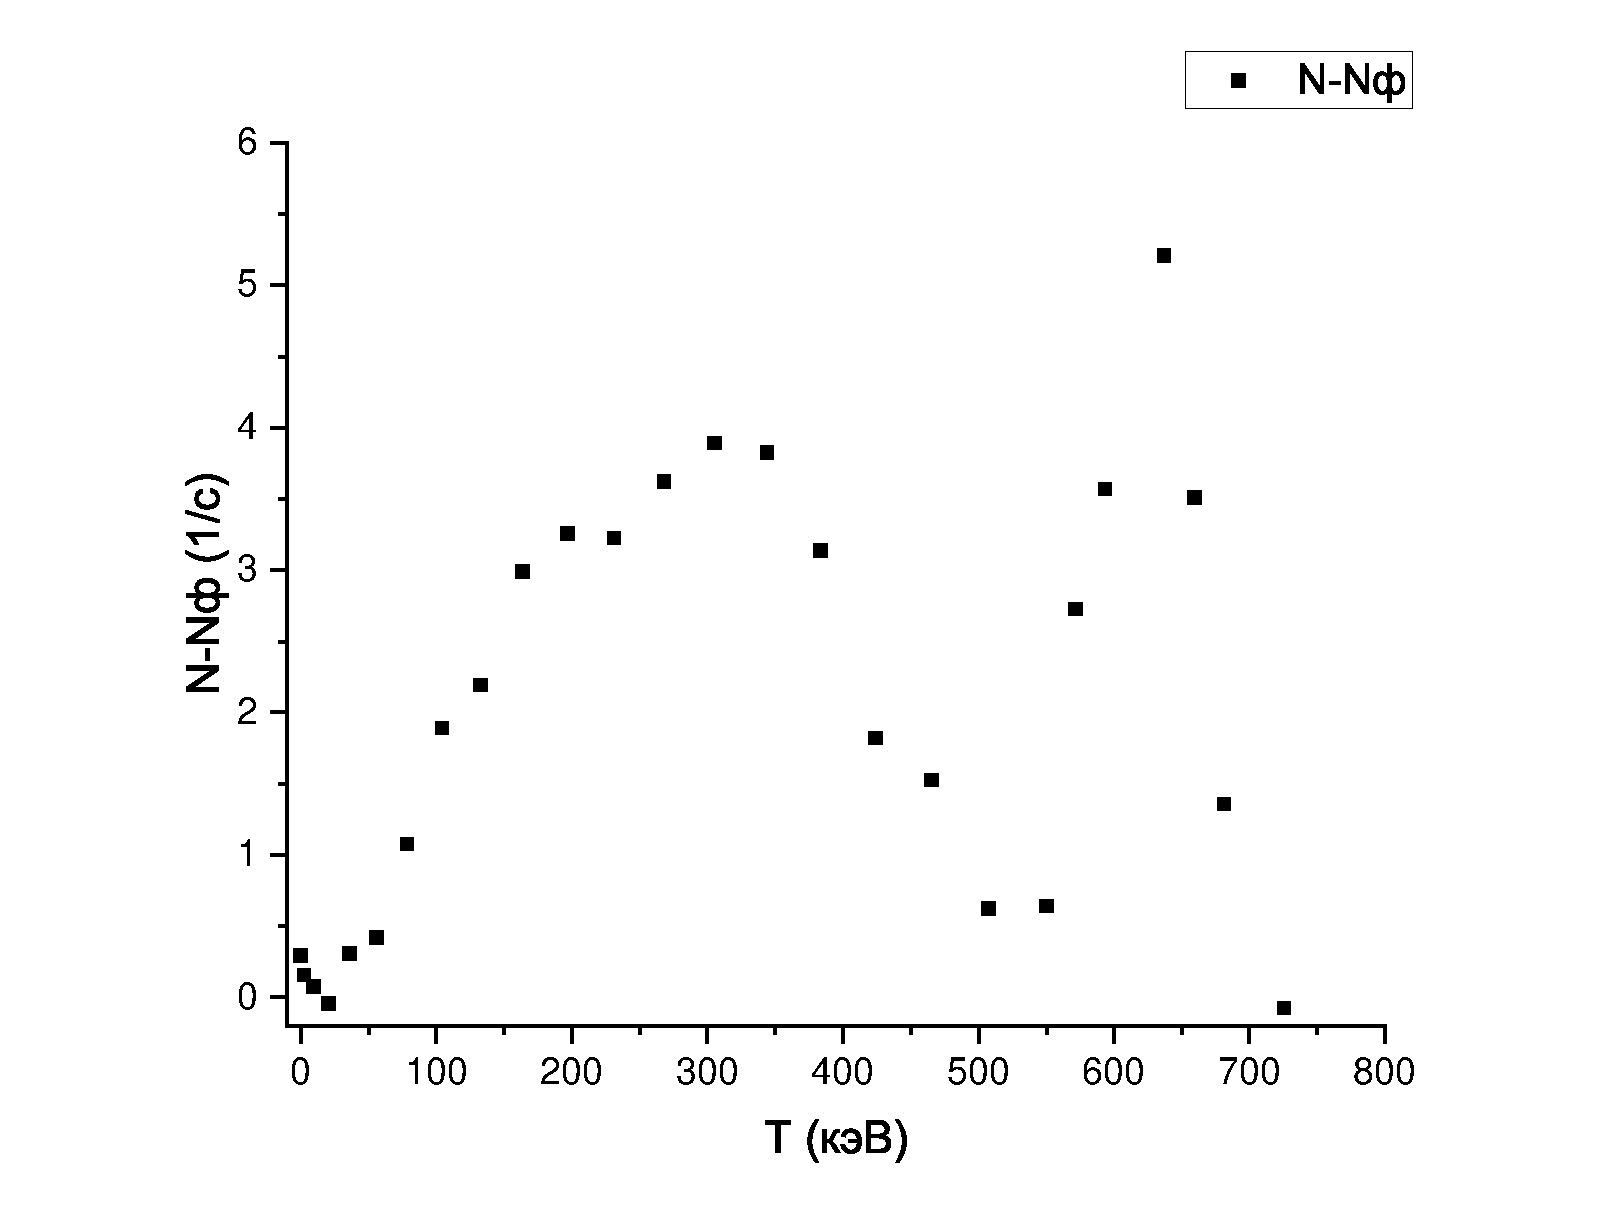
\includegraphics[width=8cm,height=7cm]{Graph3.pdf}}     
			\end{floatrow}
		\end{figure}
		
		\newpage
		Определим максимальную энергию $\beta$-спектра. Анализ рис.~\ref{fig:spectre2} в таком случае даст достаточно грубый результат, так как нам придётся ограничииться исследованием точек у самой верхней границы спектра. Эти точки измерены с наименьшей статистической точностью. Однако мы можем уменьшить ошибку определения максимальной энергии посредством процедуры Ферми-Кюри. Для этого мы отложим по оси ординат величину $\sqrt{N}/p^{3/2}$, а по оси абсцисс энергию $\beta$-частиц (с учётом того, что энергия электронов внутренней конверсии $^{137}$Cs равна 634, кэВ). В таком случае мы задействуем большинство экспериментальных точек, и прежде всего точки середины $\beta$-спектра, которые измерены с наилучшей точностью.
		
		\begin{figure}[h!]
			\begin{floatrow}
				\ffigbox[\FBwidth]{\caption{График Ферми-Кюри.}\label{fig:fermi-kuri}}%
				{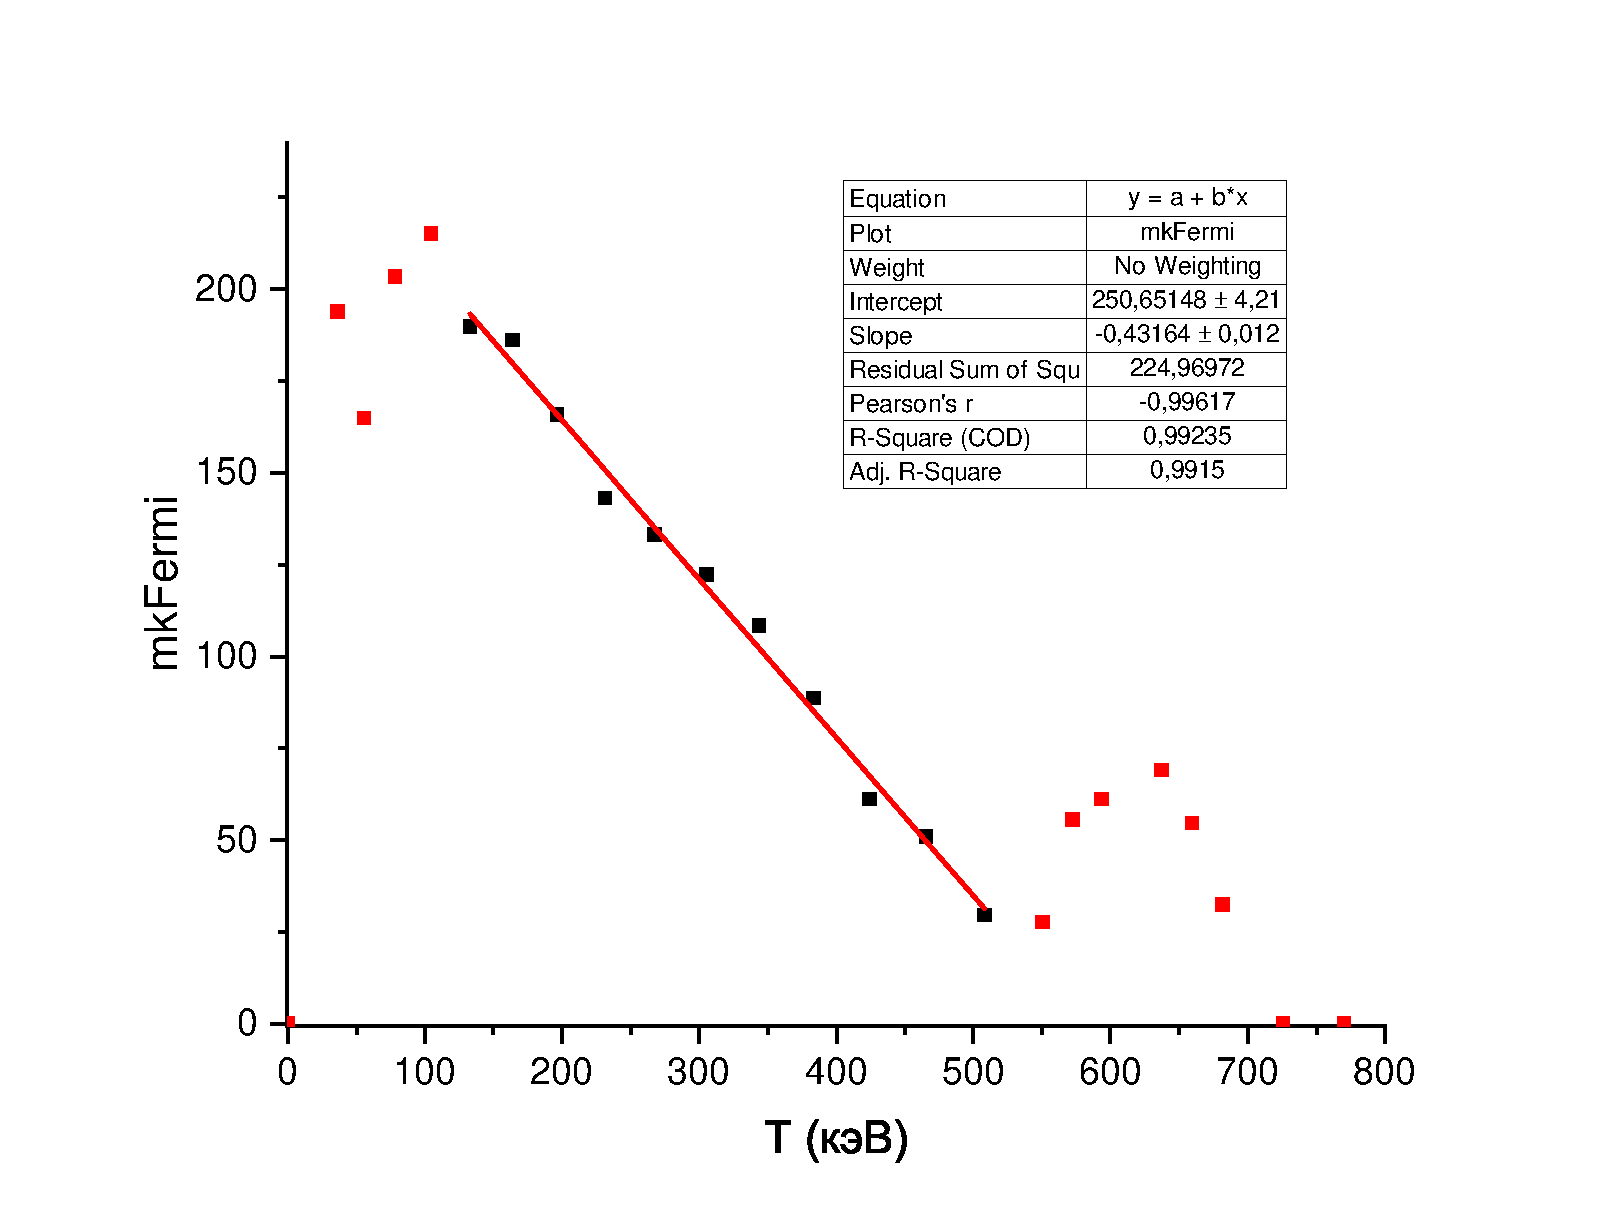
\includegraphics[width=14cm,height=10cm]{Graph2.pdf}}   
			\end{floatrow}
		\end{figure}
	
		\floatsetup[table]{capposition=top}	
		\begin{table}[H]
			\caption{Результаты линейной аппроксимации.}
			\label{table:Emax}
			\begin{tabular}{|c|c|c|}
				\hline
				& $a$ & $b$\\ \hline
							Величина    & -0,43                                                        & 251                                                                     \\ \hline
							Погрешность & 0,01                                                         & 4                                                                       \\ \hline
						\end{tabular}
		\end{table}
		Ясно, что $E_m = - \frac{b}{a}$ и $\sigma_{E_m} = E_m \sqrt{\left(\frac{\sigma_a}{a}\right)^2 + \left(\frac{\sigma_b}{b}\right)}$, откуда $E_m =(580 \pm 20) \ \text{кэВ}.$
		
	
	\section{Вывод}
	
	По результатам работы изучили энергетический спектр \btt-частиц; кроме того было получено значение максимальной энергии для электрона при \btt-распаде.

\end{document}